
% for drawing
\def\firstellip{(0, 0) ellipse [x radius=3cm, y radius=3cm, rotate=50]}
\def\bounding{(-5,-3) rectangle (5,4)}

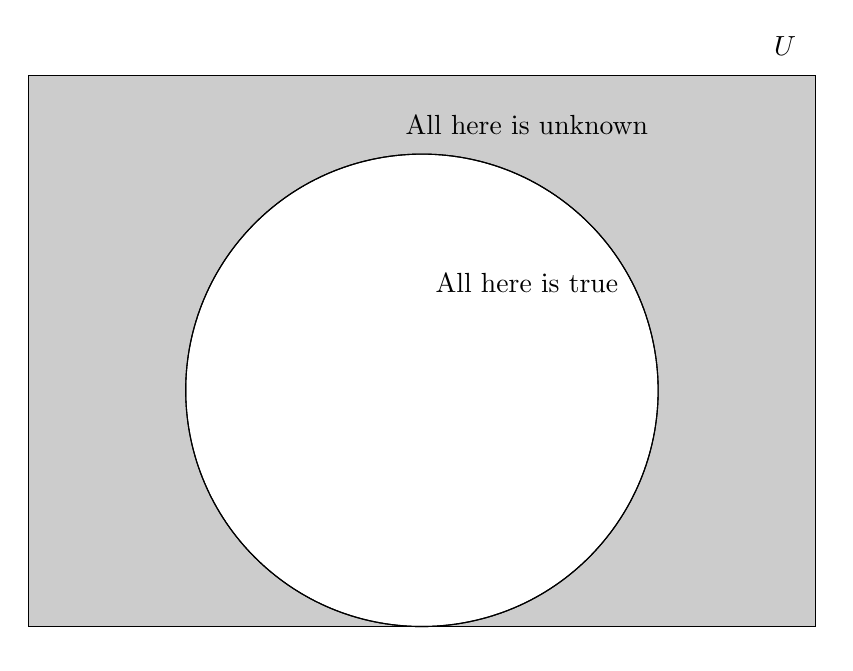
\begin{tikzpicture}

    \filldraw[fill=black, opacity=0.2] \bounding;

    %\scope \fill[white] \fourthellip; \endscope \filldraw[fill=red, opacity=0.2] \fourthellip;

    %single colors
    \scope
        \fill[white] \firstellip;
    \endscope

    \draw \firstellip node [label={[xshift=1.333cm, yshift=0.999cm]All here is true}] {};
    \draw \firstellip node [label={[xshift=1.333cm, yshift=2.999cm]All here is unknown}] {};

   % \draw \secondellip node [label={[xshift=2.2cm, yshift=2.1cm]$B$}] {};
   % \draw \thirdellip node [label={[xshift=-2.0cm, yshift=-0.9cm]$C$}] {};
   % \draw \fourthellip node [label={[xshift=-2.2cm, yshift=2.1cm]$D$}] {};
     \draw \bounding node [label=above left:$U$] {};

   % \begin{scope}
   %     \begin{scope}[even odd rule]% first ellipse corner
   %         \clip \secondellip (-5,-5) rectangle (5,5);
   %         \clip \thirdellip (-5,-5) rectangle (5,5);
   %         \clip \fourthellip (-5,-5) rectangle (5,5);
   %     \fill[yellow] \firstellip;
   %     \end{scope}
   % \end{scope}

   % \begin{scope}
   %     \begin{scope}[even odd rule]% second ellipse corner
   %         \clip \firstellip (-5,-5) rectangle (5,5);
   %         \clip \thirdellip (-5,-5) rectangle (5,5);
   %         \clip \fourthellip (-5,-5) rectangle (5,5);
   %     \fill[yellow] \secondellip;
   %     \end{scope}
   % \end{scope}

   % \begin{scope}
   %     \begin{scope}[even odd rule]% third ellipse corner
   %         \clip \secondellip (-5,-5) rectangle (5,5);
   %         \clip \firstellip (-5,-5) rectangle (5,5);
   %         \clip \fourthellip (-5,-5) rectangle (5,5);
   %     \fill[yellow] \thirdellip;
   %     \end{scope}
   % \end{scope}

\end{tikzpicture}
